\documentclass[conference,a4paper]{IEEEtran}
\IEEEoverridecommandlockouts

\usepackage[indonesian]{babel}
\usepackage[utf8]{inputenc}
\usepackage{float}
\usepackage{placeins}
\usepackage[T1]{fontenc}
\usepackage{cite}
\usepackage{amsmath,amssymb}
\usepackage{graphicx}
\usepackage{booktabs}
\usepackage{siunitx}
\usepackage{xcolor}
\usepackage[hidelinks]{hyperref}
\graphicspath{{gambar/}}

\newcommand{\petunjuk}[1]{\textcolor{gray}{[#1]}}

\begin{document}

\title{Studi Ablasi RNN, LSTM, dan GRU dibandingkan ANN untuk Prediksi Trafik Seluler Kota Milan}

\author{
 \IEEEauthorblockN{Shintya Linsi Nainggolan}
\IEEEauthorblockA{NIM 124400049\\
Teknik Telekomunikasi, ITERA\\
shintya.124400049@student.itera.ac.id}
\and
}

\maketitle

\begin{abstract}
Prediksi trafik internet seluler merupakan salah satu kebutuhan penting dalam pengelolaan jaringan telekomunikasi untuk mengantisipasi perubahan beban jaringan dan meningkatkan efisiensi penggunaan sumber daya. Penelitian ini membandingkan kinerja Artificial Neural Network (ANN), Recurrent Neural Network (RNN), Long Short-Term Memory (LSTM), dan Gated Recurrent Unit (GRU) dalam memprediksi trafik internet per jam menggunakan dataset Telecom Italia Milan. Eksperimen dilakukan pada wilayah Duomo dan lokasi kelompok Corso Como melalui studi ablasi terhadap panjang jendela waktu, jumlah hidden unit, jumlah lapisan, learning rate, kombinasi fitur, batch size, dan dropout. Setiap konfigurasi dievaluasi menggunakan tiga random seed dengan Mean Absolute Error (MAE) sebagai metrik utama. Pemilihan hyperparameter dilakukan berdasarkan rata-rata MAE validasi. Hasil pengujian di Duomo menunjukkan bahwa GRU memperoleh MAE validasi terendah sebesar 188,65. Sementara itu, pada pengujian generalisasi di Corso Como, LSTM dengan konfigurasi terpilih menghasilkan MAE validasi sebesar 131,1 dan MAE pengujian sebesar 119,2. Hasil penelitian menunjukkan bahwa pemilihan hyperparameter dan karakteristik trafik setiap lokasi memengaruhi akurasi prediksi, sehingga konfigurasi yang optimal pada suatu lokasi belum tentu memberikan kinerja terbaik pada lokasi lainnya.
\end{abstract}

\begin{IEEEkeywords}
prediksi trafik seluler, RNN, LSTM, GRU, studi ablasi
\end{IEEEkeywords}

% ---------------------------------------------------------------------
\section{Pendahuluan}
Prediksi trafik internet per sel diperlukan operator telekomunikasi untuk mengantisipasi perubahan beban jaringan dan mengoptimalkan alokasi sumber daya. Artificial Neural Network (ANN) mampu mempelajari hubungan antarfitur, tetapi tidak secara khusus memodelkan ketergantungan waktu. Sebaliknya, Recurrent Neural Network (RNN) memproses informasi berurutan, sedangkan Long Short-Term Memory (LSTM) \cite{hochreiter1997lstm} dan Gated Recurrent Unit (GRU) \cite{cho2014gru} menggunakan mekanisme gerbang untuk mengelola informasi temporal.

Studi ablasi dilakukan untuk mengidentifikasi pengaruh masing-masing hyperparameter terhadap akurasi prediksi. Kontribusi laporan ini meliputi:
\begin{enumerate}
\item Menganalisis pengaruh panjang jendela, hidden unit, jumlah lapisan, learning rate, fitur, batch size, dan dropout terhadap performa ANN, RNN, LSTM, dan GRU.
\item Menentukan konfigurasi berdasarkan MAE validasi serta mengevaluasi generalisasinya dari Duomo ke Corso Como.
\end{enumerate}

% ---------------------------------------------------------------------
\section{Data dan Metode}
\subsection{Dataset}
Penelitian ini menggunakan dataset trafik seluler Kota Milan yang berasal dari Telecom Italia Big Data Challenge \cite{barlacchi2015milan}. Data yang digunakan mencakup periode November--Desember 2013 dengan resolusi waktu satu jam. Dataset memuat informasi aktivitas komunikasi seluler berupa trafik internet (net), panggilan (call), dan pesan singkat (sms). Selain itu, informasi waktu berupa jam dan hari dikonversi menjadi representasi siklik menggunakan fungsi sinus dan kosinus, sehingga diperoleh tujuh fitur, yaitu net, call, sms, jam\_sin, jam\_cos, hari\_sin, dan hari\_cos. Variabel net digunakan sebagai target prediksi trafik internet per jam.

Eksperimen dilakukan pada dua lokasi di Kota Milan. Lokasi pertama adalah Duomo dengan nomor kotak 5060 yang digunakan sebagai lokasi acuan untuk pengujian model dan studi ablasi. Lokasi kedua adalah Corso Como dengan kode lokasi kelompok 9 dan nomor kotak 5859 yang digunakan untuk menguji kemampuan generalisasi model. Kedua lokasi digunakan untuk menganalisis perbedaan karakteristik trafik internet serta pengaruhnya terhadap akurasi prediksi.

\begin{figure}[H]
  \centering
  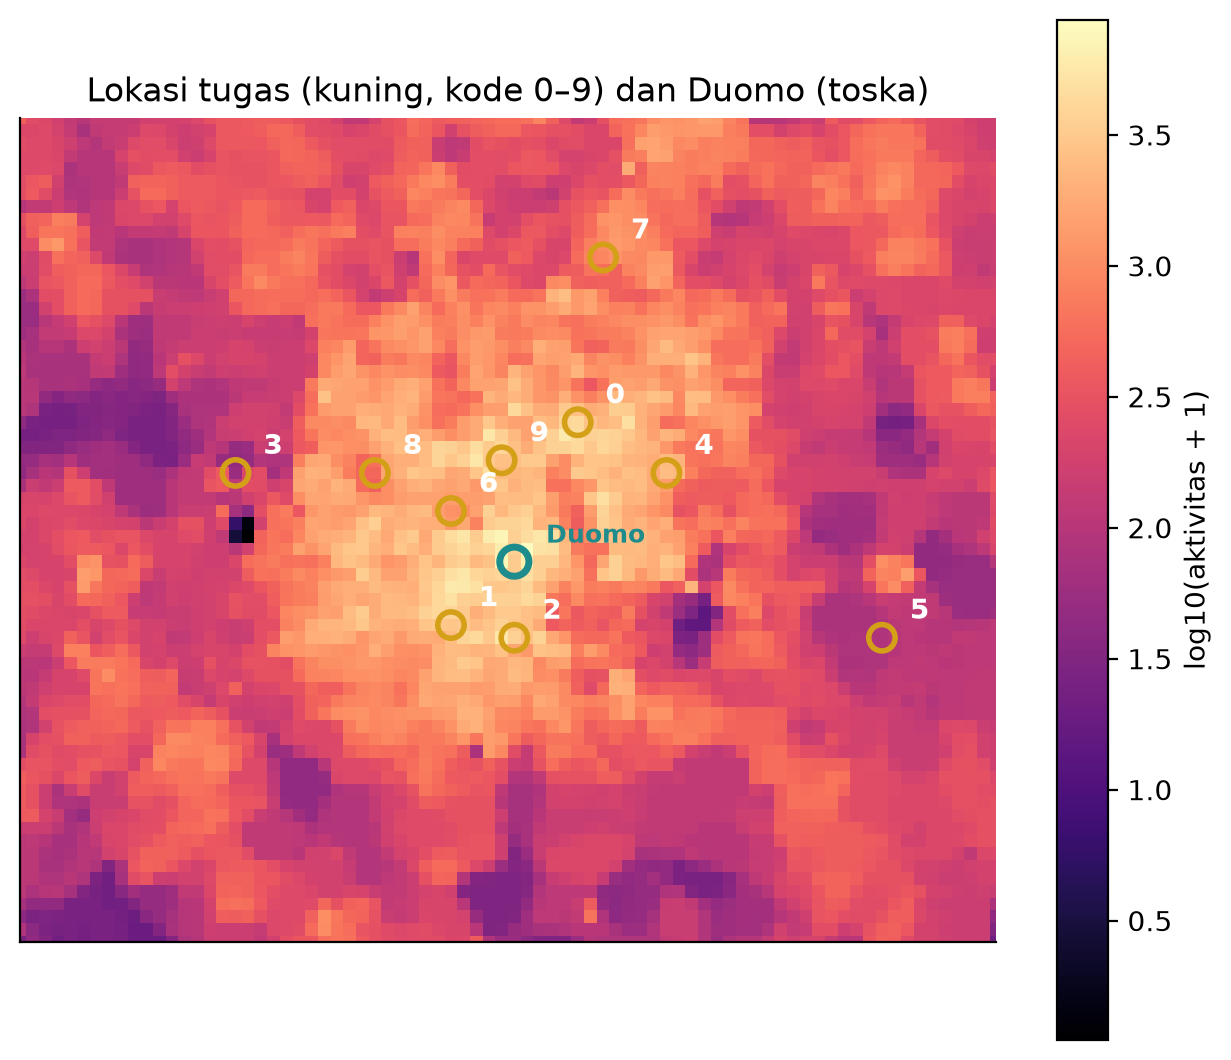
\includegraphics[width=0.85\linewidth]{peta_lokasi_tugas.png}
  \caption{Rata-rata aktivitas internet per kotak di Milan. Lingkaran kuning: lokasi tugas (kode 0--9); lingkaran toska: Duomo.}
  \label{fig:peta}
\end{figure}

\subsection{Pembagian Data dan Praproses}

Dataset dibagi secara kronologis menjadi empat periode, yaitu data pelatihan pada 11 November--8 Desember 2013, data validasi pada 9--15 Desember 2013, data pengujian pada 16--22 Desember 2013, serta periode Natal mulai 23 Desember 2013. Standardisasi dilakukan menggunakan rata-rata dan simpangan baku yang dihitung hanya dari data pelatihan sebelum 9 Desember 2013. Statistik tersebut kemudian diterapkan pada data validasi, pengujian, dan periode Natal agar informasi dari masa depan tidak memengaruhi proses pelatihan.

Pembentukan data masukan menggunakan teknik \textit{sliding window}, yaitu mengambil $W$ pengamatan sebelumnya untuk memprediksi trafik internet pada horizon $H$ jam berikutnya. Konfigurasi acuan menggunakan panjang jendela $W=24$ jam dan horizon prediksi $H=1$ jam. Setiap sampel dikelompokkan berdasarkan waktu target prediksinya. Pembagian data dilakukan secara kronologis tanpa mengacak urutan periode waktu untuk mencegah kebocoran informasi (\textit{data leakage}) dari data masa depan ke proses pelatihan. Dengan demikian, evaluasi model dapat menggambarkan kemampuan prediksi terhadap data yang belum pernah digunakan dalam pelatihan secara lebih realistis.

\subsection{Model dan Konfigurasi Acuan}
Penelitian ini membandingkan empat arsitektur jaringan saraf, yaitu Artificial Neural Network (ANN), Recurrent Neural Network (RNN), Long Short-Term Memory (LSTM), dan Gated Recurrent Unit (GRU). ANN digunakan sebagai model pembanding yang mempelajari hubungan antarfitur tanpa mekanisme memori rekuren. RNN memproses data secara berurutan dengan memanfaatkan informasi dari langkah waktu sebelumnya. LSTM menggunakan mekanisme gerbang untuk mempertahankan informasi penting dalam urutan yang panjang, sedangkan GRU menerapkan mekanisme gerbang yang lebih sederhana untuk mengatur aliran informasi.

Keempat model diuji menggunakan konfigurasi acuan yang mencakup panjang jendela waktu, horizon prediksi, jumlah hidden unit, jumlah lapisan, fitur masukan, optimizer, learning rate, batch size, dan early stopping. Konfigurasi tersebut digunakan sebagai dasar perbandingan sebelum dilakukan studi ablasi. Rincian hyperparameter acuan disajikan pada Tabel~\ref{tab:acuan}.

\begin{table}[H]
  \centering
  \caption{Konfigurasi acuan}
  \label{tab:acuan}
  \begin{tabular}{@{}ll@{}}
    \toprule
    Hyperparameter & Nilai acuan \\
    \midrule
    Panjang jendela $W$ & 24 jam \\
    Horizon & 1 jam \\
    Ukuran hidden & ANN 32, RNN 68, LSTM 33, GRU 38 \\
    Jumlah lapisan & ANN 2, rekuren 1 \\
    Fitur & 3 trafik + 4 fitur waktu siklik (7) \\
    Optimizer, \textit{learning rate} & Adam, $10^{-3}$ \\
    \textit{Batch size} & 64 \\
    \textit{Early stopping} & \textit{patience} 30, maks.\ 300 epoch \\
    \bottomrule
  \end{tabular}
\end{table}

\subsection{Protokol Ablasi dan Evaluasi}
Studi ablasi dilakukan dengan mengubah satu faktor pada setiap percobaan, sedangkan parameter lainnya dipertahankan sesuai konfigurasi acuan. Bagian A mencakup lima faktor, yaitu A1 panjang jendela waktu (6, 12, 24, 48, dan 168 jam), A2 ukuran hidden (16, 32, 64, dan 128), A3 jumlah lapisan (1, 2, dan 3), A4 learning rate (0,0001; 0,001; dan 0,01), serta A5 kelompok fitur (net, net+call+sms, net+waktu, dan semua).

Hipotesis awal penelitian adalah bahwa panjang jendela dan ukuran hidden yang sesuai dapat meningkatkan akurasi prediksi, sedangkan penambahan lapisan dan learning rate yang terlalu besar belum tentu menghasilkan kinerja lebih baik. Penggunaan fitur waktu diperkirakan membantu model mengenali pola trafik internet secara periodik.

Pada Bagian B, dipilih dua faktor tambahan, yaitu B1 batch size (16, 64, dan 256) serta B2 dropout (0; 0,2; dan 0,5). Kedua faktor dipilih untuk mengevaluasi pengaruh proses optimasi dan regularisasi. Hipotesis awalnya adalah batch size kecil memungkinkan pembaruan parameter lebih sering, sedangkan dropout sedang berpotensi mengurangi overfitting.

Setiap konfigurasi dijalankan menggunakan tiga random seed (0, 1, dan 2). Hasil evaluasi dilaporkan dalam bentuk rata-rata dan simpangan baku. Metrik yang digunakan meliputi Mean Absolute Error (MAE), Root Mean Squared Error (RMSE), dan Mean Absolute Percentage Error (MAPE) pada skala asli data. Konfigurasi terbaik dipilih berdasarkan rata-rata MAE validasi, bukan MAE pengujian. Seluruh eksperimen dijalankan menggunakan PyTorch pada CPU. Berdasarkan catatan 372 run eksperimen, total waktu pelatihan yang terakumulasi adalah 1169,5 menit.

% ---------------------------------------------------------------------
\section{Hasil}

\subsection{Baseline Naif dan Acuan}
Eksperimen awal dilakukan pada lokasi Duomo untuk membandingkan tiga metode baseline naif dengan empat model pembelajaran mendalam, yaitu ANN, RNN, LSTM, dan GRU. Baseline naif terdiri atas prediksi berdasarkan nilai pada hari sebelumnya, minggu sebelumnya, dan nilai terakhir yang diamati. Perbandingan utama menggunakan horizon prediksi satu jam sesuai konfigurasi acuan. Hasil evaluasi ditampilkan pada Tabel~\ref{tab:baseline}.

\begin{table}[H]
\centering
\caption{Perbandingan baseline naif dan model acuan pada lokasi Duomo (horizon 1 jam)}
\label{tab:baseline}
\scriptsize
\begin{tabular}{@{}lcc@{}}
\toprule
Metode & Val. MAE & Test MAE \\
\midrule
Naif: kemarin & $595{,}3$ & $552{,}2$ \\
Naif: minggu lalu & $492{,}8$ & $467{,}6$ \\
Naif: nilai terakhir & $662{,}6$ & $600{,}9$ \\
\midrule
ANN & $250{,}1\pm8{,}6$ & $313{,}9\pm9{,}9$ \\
RNN & $206{,}1\pm7{,}4$ & $229{,}6\pm5{,}1$ \\
LSTM & $230{,}5\pm12{,}2$ & $273{,}6\pm25{,}4$ \\
GRU & $207{,}5\pm3{,}8$ & $237{,}2\pm9{,}3$ \\
\bottomrule
\end{tabular}
\end{table}

Berdasarkan hasil pengujian, baseline naif minggu lalu menghasilkan MAE terendah di antara metode naif, yaitu 467,6. Sementara itu, seluruh model pembelajaran mendalam menghasilkan kesalahan prediksi yang lebih kecil. Model RNN memperoleh kinerja terbaik pada konfigurasi acuan dengan rata-rata Test MAE sebesar 229,6, diikuti GRU sebesar 237,2, LSTM sebesar 273,6, dan ANN sebesar 313,9.

Pada data validasi, RNN juga memperoleh MAE terendah sebesar 206,1, meskipun nilainya berdekatan dengan GRU sebesar 207,5. Hasil ini menunjukkan bahwa pemodelan hubungan temporal menggunakan arsitektur rekuren lebih efektif daripada ANN pada konfigurasi acuan untuk prediksi trafik internet Duomo. Nilai pada model pembelajaran mendalam disajikan sebagai rata-rata $\pm$ simpangan baku dari tiga random seed.


\subsection{Ablasi Wajib}

\begin{figure*}[!t]
\centering
\setlength{\tabcolsep}{4pt}
\renewcommand{\arraystretch}{1.2}

\begin{tabular}{@{}cc@{}}

% A1 - Panjang Jendela
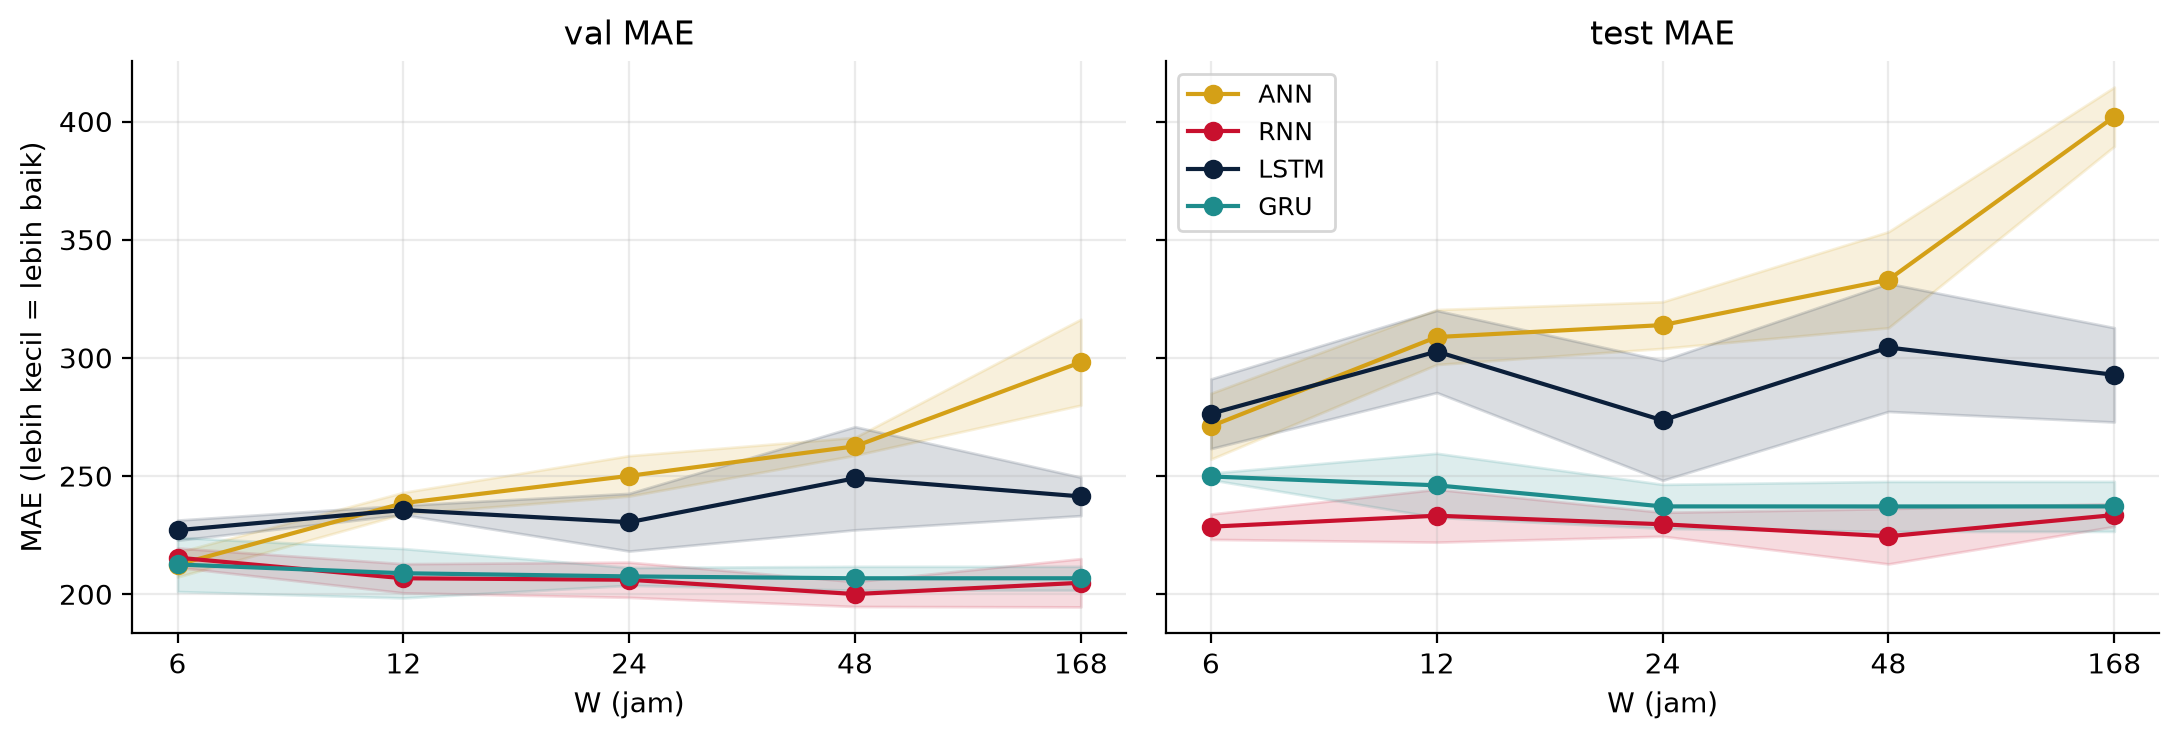
\includegraphics[width=0.45\textwidth,height=3cm,keepaspectratio]{gambar/A1_W.png}
&
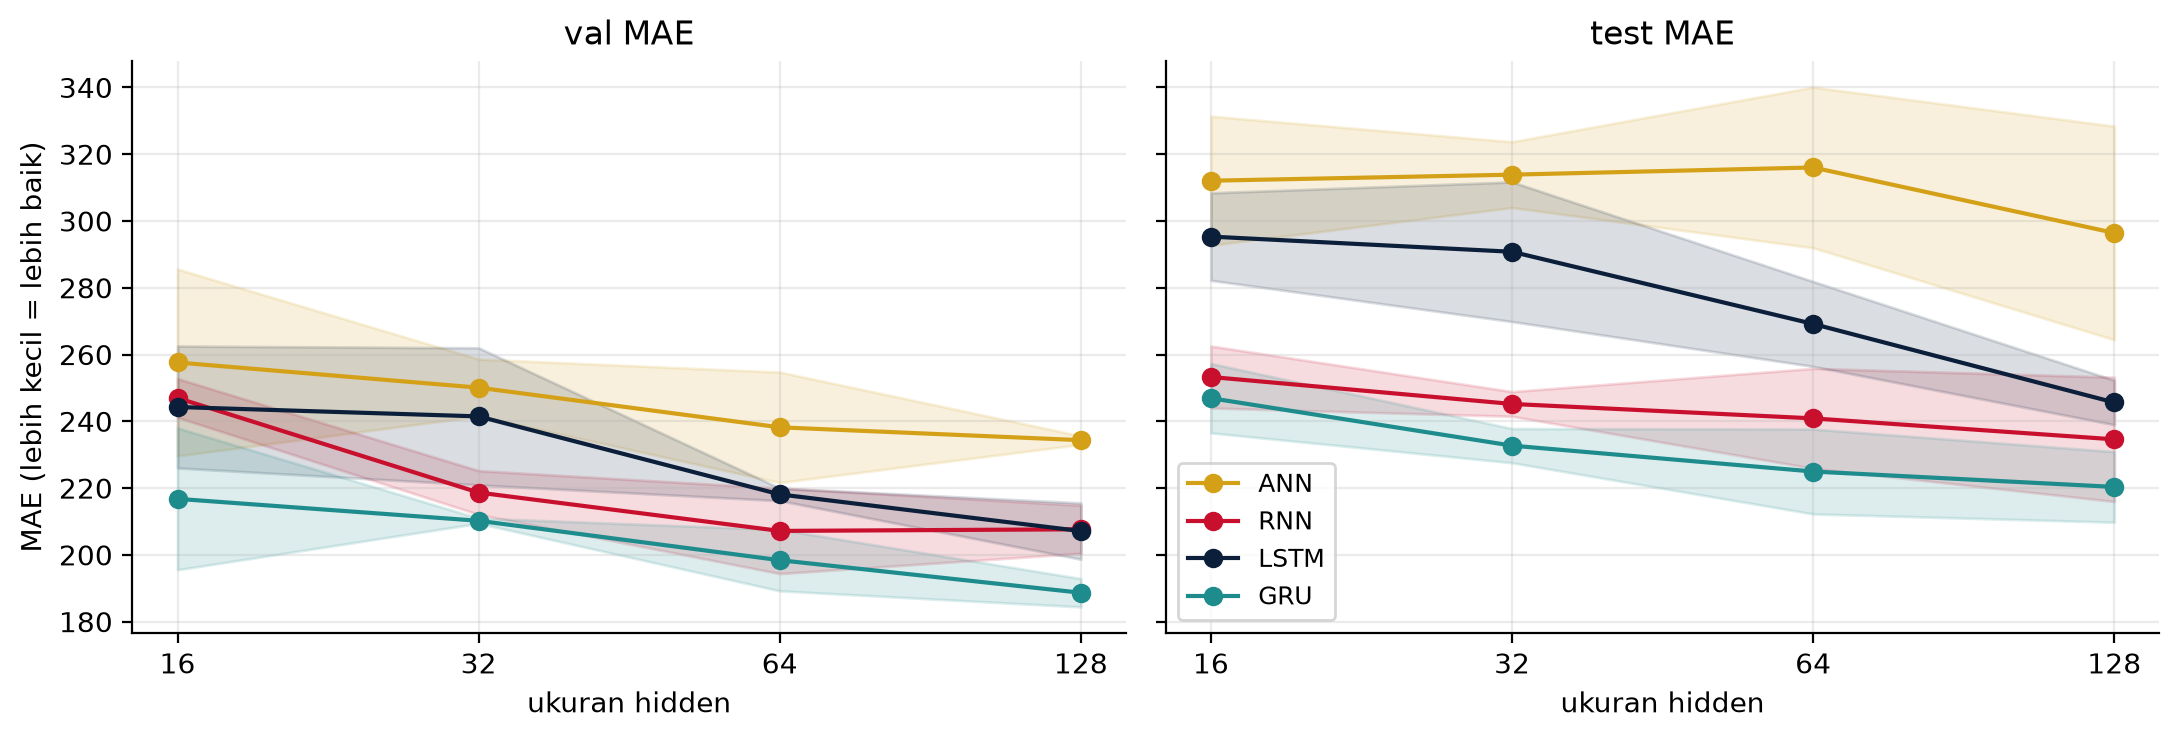
\includegraphics[width=0.45\textwidth,height=3cm,keepaspectratio]{gambar/A2_hidden.png}
\\

{\footnotesize\textbf{Gambar 2(a).} A1: Pengaruh Panjang Jendela $W$}
&
{\footnotesize\textbf{Gambar 2(b).} A2: Pengaruh Ukuran Hidden}
\\[2mm]

% A2 - Jumlah Parameter dan A3 - Jumlah Lapisan
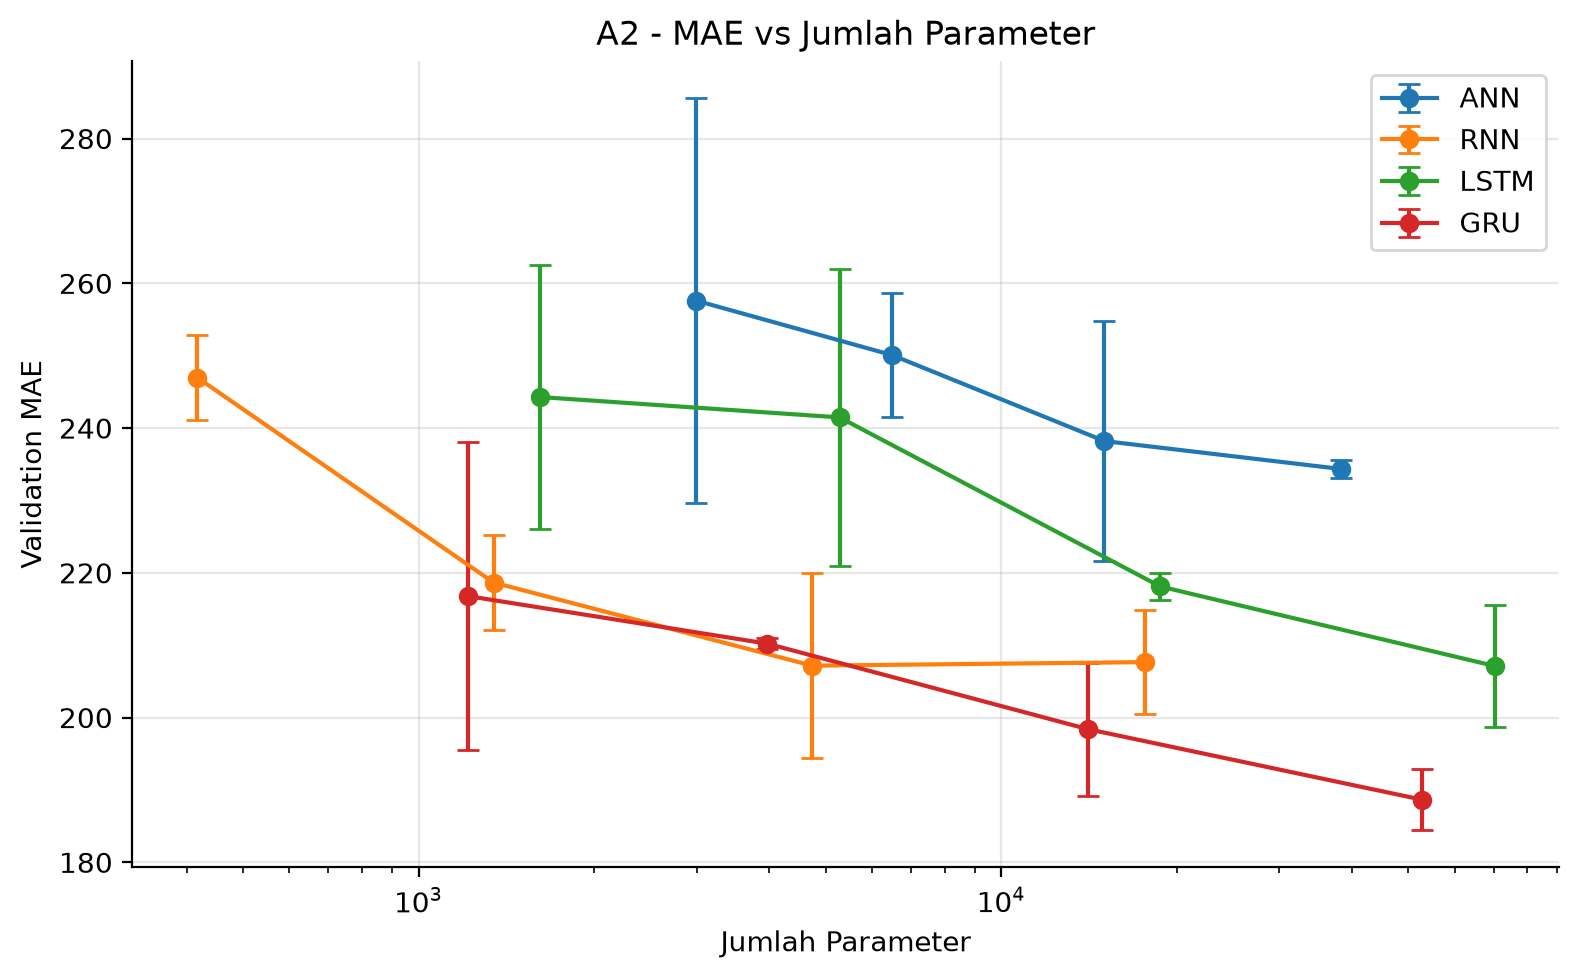
\includegraphics[width=0.45\textwidth,height=3cm,keepaspectratio]{gambar/A2_MAE_vs_param.png}
&
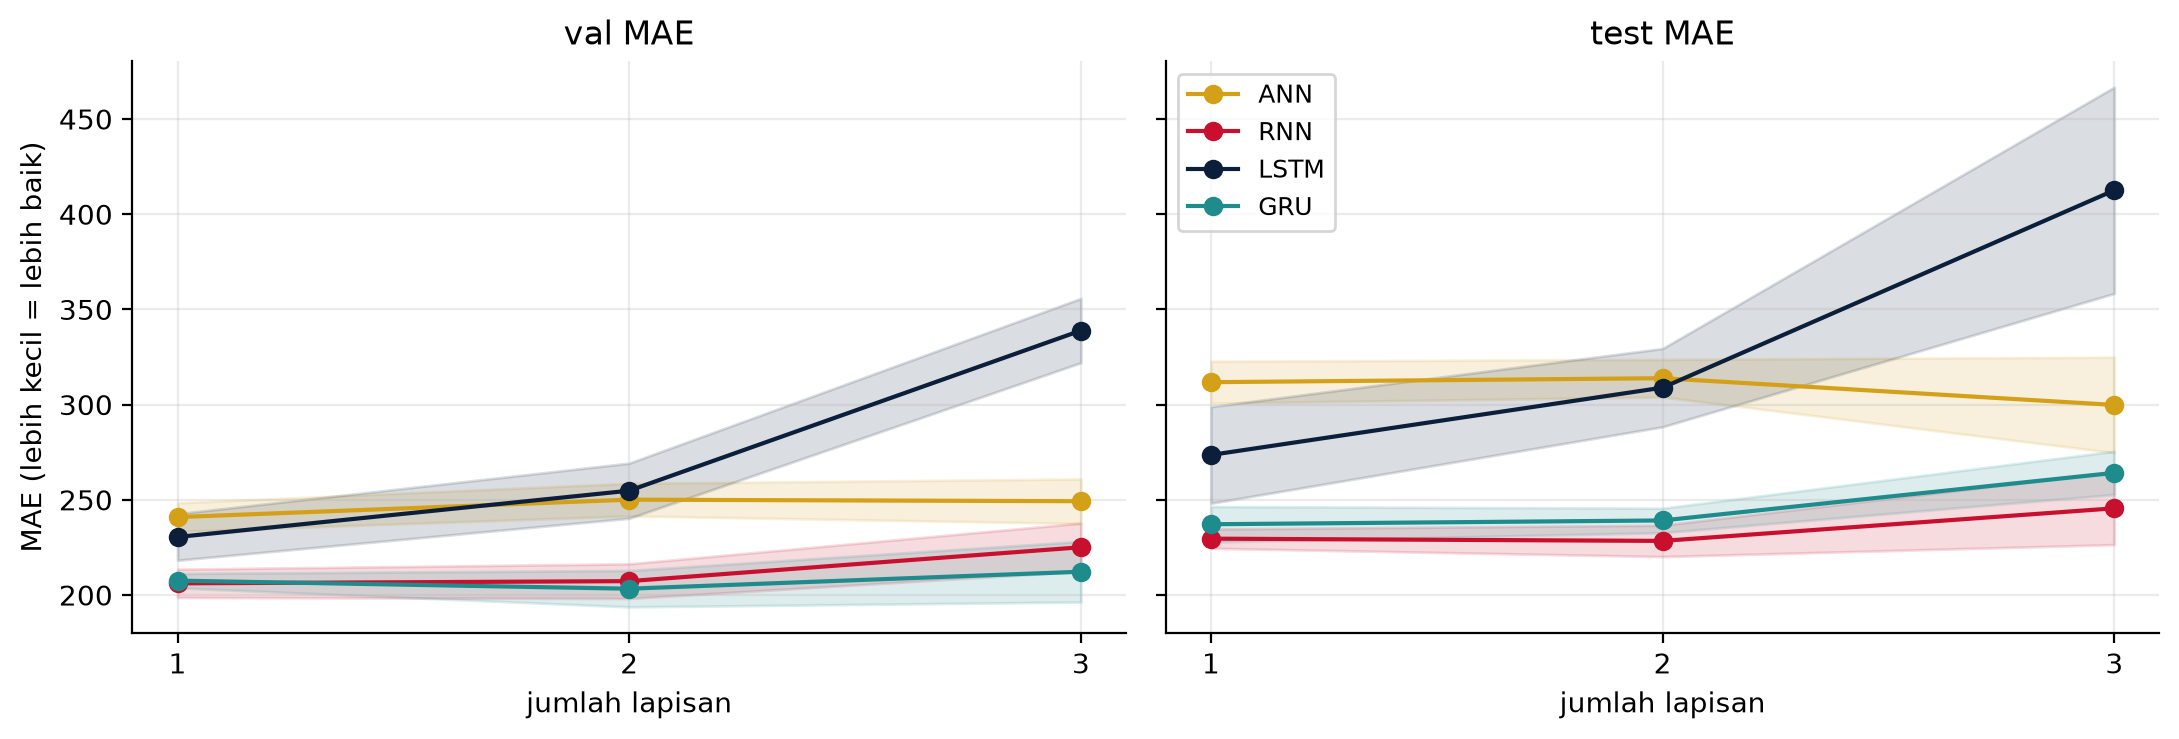
\includegraphics[width=0.45\textwidth,height=3cm,keepaspectratio]{gambar/A3_layers.png}
\\

{\footnotesize\textbf{Gambar 2(c).} A2: MAE Validasi vs Jumlah Parameter}
&
{\footnotesize\textbf{Gambar 2(d).} A3: Pengaruh Jumlah Lapisan}
\\[2mm]

% A4 - Learning Rate dan A5 - Kelompok Fitur
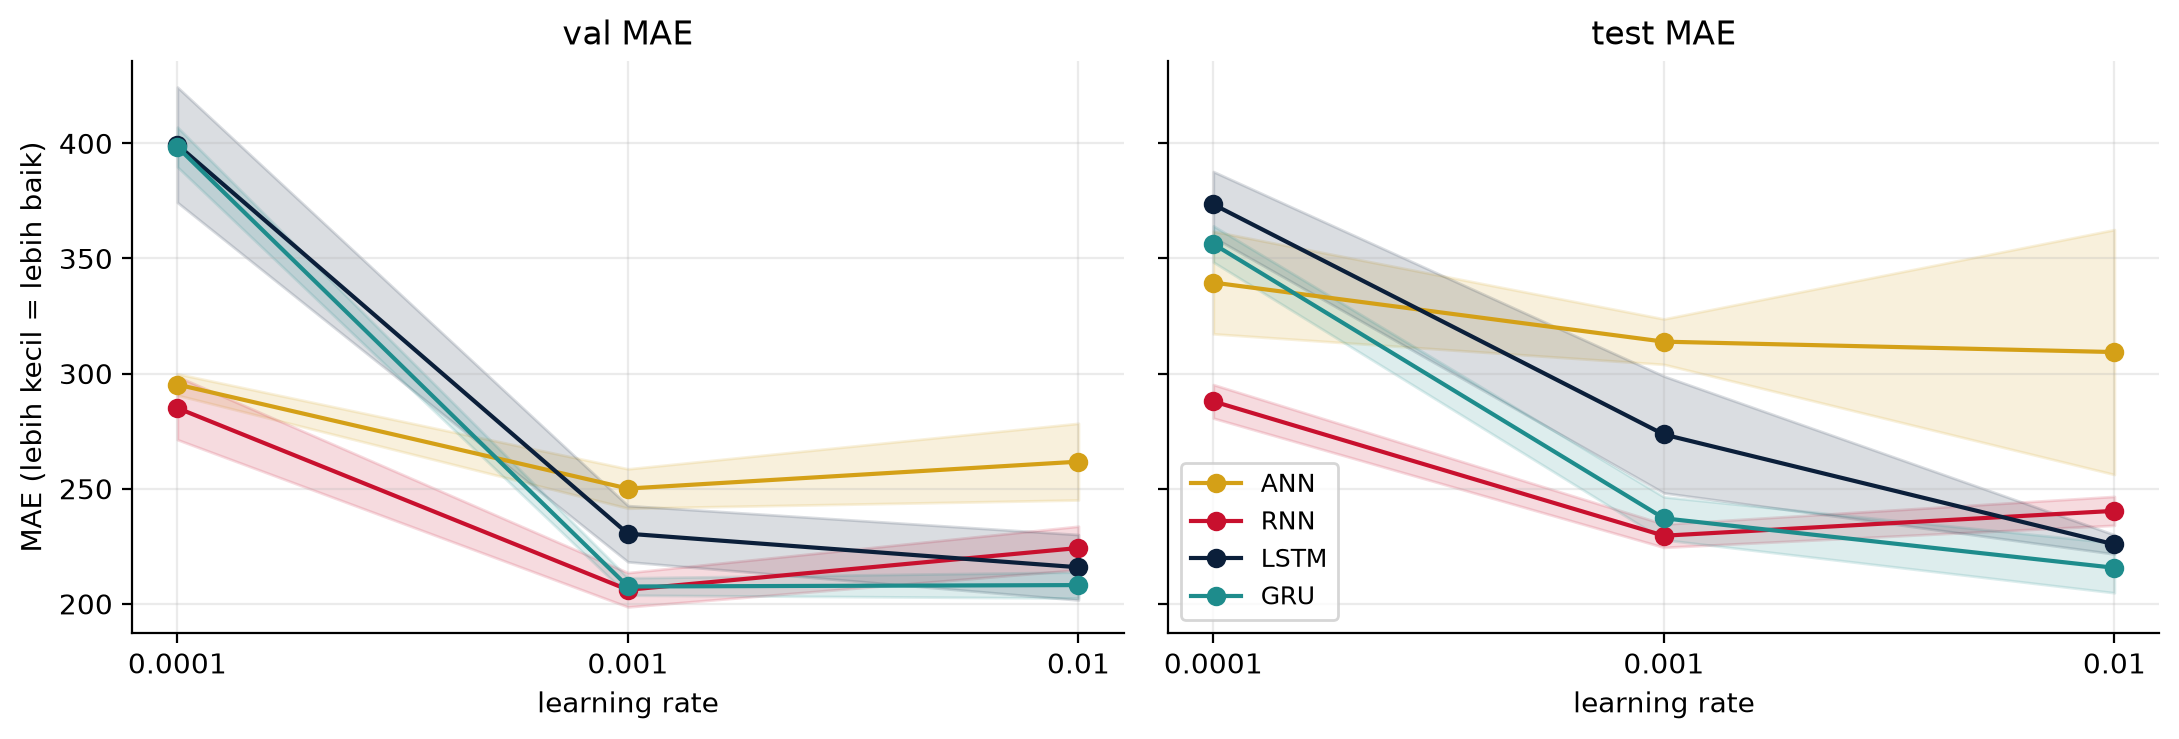
\includegraphics[width=0.45\textwidth,height=3cm,keepaspectratio]{gambar/A4_lr.png}
&
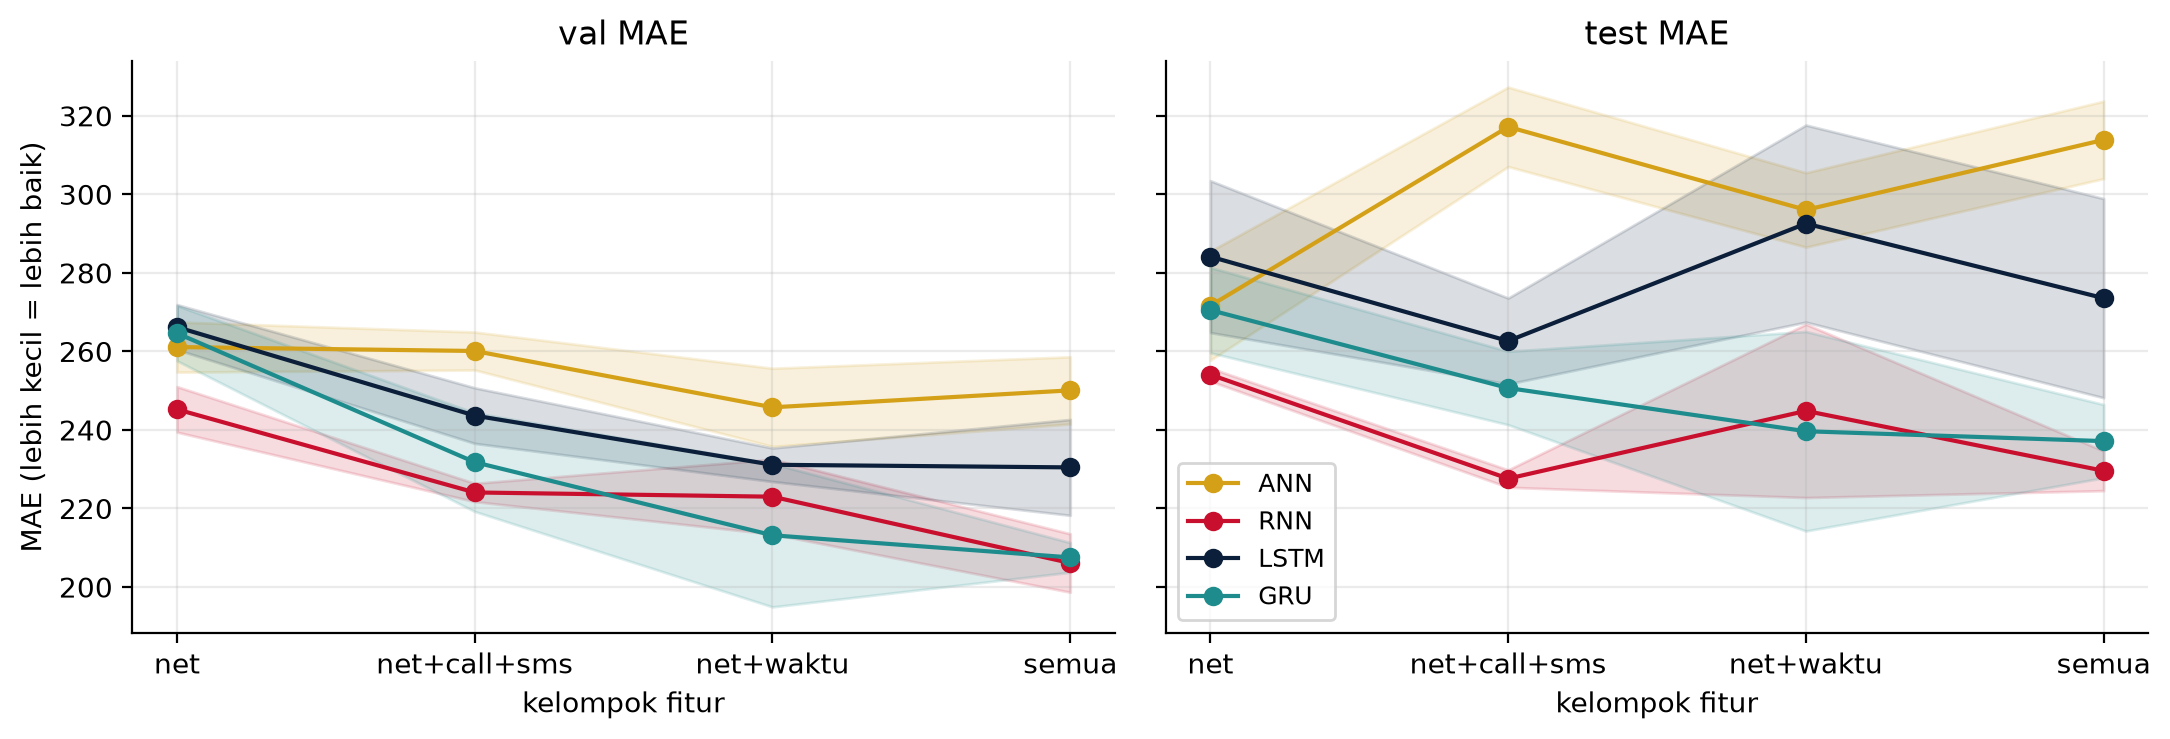
\includegraphics[width=0.45\textwidth,height=3cm,keepaspectratio]{gambar/A5_fitur.png}
\\

{\footnotesize\textbf{Gambar 2(e).} A4: Pengaruh Learning Rate}
&
{\footnotesize\textbf{Gambar 2(f).} A5: Pengaruh Kelompok Fitur}

\end{tabular}

\caption{Hasil studi ablasi wajib A1--A5 yang memperlihatkan pengaruh panjang jendela, ukuran hidden, jumlah parameter, jumlah lapisan, learning rate, dan kelompok fitur terhadap kinerja model ANN, RNN, LSTM, dan GRU.}
\label{fig:ablasiA}
\label{fig:ablasi_wajib}

\end{figure*}

\begin{table}[H]
\centering
\caption{Test MAE pada variasi panjang jendela di Duomo (rata-rata $\pm$ simpangan baku, tiga seed)}
\label{tab:ablasiA1}
\scriptsize
\resizebox{\columnwidth}{!}{%
\begin{tabular}{@{}lcccc@{}}
\toprule
$W$ (jam) & ANN & RNN & LSTM & GRU \\
\midrule
6 & $271{,}1\pm13{,}9$ & $228{,}6\pm5{,}4$ & $276{,}3\pm14{,}7$ & $249{,}8\pm1{,}4$ \\
12 & $308{,}8\pm11{,}6$ & $233{,}2\pm11{,}2$ & $302{,}7\pm17{,}4$ & $246{,}1\pm13{,}5$ \\
24 & $313{,}9\pm9{,}9$ & $229{,}6\pm5{,}1$ & $273{,}6\pm25{,}4$ & $237{,}2\pm9{,}3$ \\
48 & $333{,}1\pm20{,}3$ & $224{,}5\pm11{,}7$ & $304{,}4\pm27{,}1$ & $237{,}1\pm10{,}6$ \\
168 & $402{,}0\pm12{,}5$ & $233{,}5\pm4{,}8$ & $292{,}8\pm20{,}0$ & $237{,}2\pm10{,}6$ \\
\bottomrule
\end{tabular}%
}
\end{table}

\subsubsection{A1: Panjang Jendela}

Berdasarkan Gambar~\ref{fig:ablasiA}(a) dan Tabel~\ref{tab:ablasiA1},, panjang jendela $W=\{6,12,24,48,168\}$ jam yang semakin besar tidak selalu meningkatkan akurasi prediksi. ANN menjadi model paling sensitif karena Test MAE meningkat dari 271,1 pada $W=6$ menjadi 402,0 pada $W=168$. Jumlah parameter ANN juga meningkat dari 2.465 menjadi 38.753, sehingga kompleksitas model dan risiko \textit{overfitting} bertambah. Sebaliknya, model rekuren memiliki jumlah parameter tetap karena bobot digunakan berulang pada setiap langkah waktu. RNN mencapai Test MAE terendah sebesar 224,5 pada $W=48$.

Hasil ini sejalan dengan eksperimen pengaruh setiap jam masukan pada Workshop Deep Learning Sesi 2. Pengaruh masukan dari 24 jam sebelumnya hanya sekitar 1\%, sedangkan dari 168 jam sebelumnya mendekati nol. Dengan demikian, informasi historis yang lebih panjang tidak selalu memberikan manfaat tambahan untuk prediksi trafik satu jam ke depan.

\subsubsection{A2: Ukuran Hidden}

Berdasarkan Gambar~\ref{fig:ablasiA}(b), peningkatan ukuran \textit{hidden} tidak selalu menghasilkan akurasi yang lebih baik. Pada GRU, Validation MAE menurun dari 216,8 saat \textit{hidden} 16 menjadi 188,7 saat \textit{hidden} 128. Namun, RNN pada \textit{hidden} 64 dan 128 menunjukkan Validation MAE yang hampir sama, yaitu 207,2 dan 207,7. Hal ini menunjukkan bahwa penambahan kapasitas model tidak selalu memberikan peningkatan kinerja yang sebanding.

Perbandingan MAE terhadap jumlah parameter pada Gambar~\ref{fig:ablasiA}(c) memperlihatkan bahwa ukuran \textit{hidden} yang sama tidak menghasilkan kompleksitas setara. Pada \textit{hidden} 64, LSTM mempunyai 18.753 parameter, sedangkan RNN hanya 4.737 parameter. Walaupun memiliki parameter lebih banyak, Validation MAE LSTM sebesar 218,1 masih lebih tinggi daripada RNN sebesar 207,2. Dengan jumlah data latih sekitar 672 sampel, model yang lebih kompleks tidak selalu menghasilkan generalisasi lebih baik.

\subsubsection{A3: Jumlah Lapisan}

Berdasarkan Gambar~\ref{fig:ablasiA}(d), penambahan jumlah lapisan rekuren tidak selalu meningkatkan akurasi. LSTM mengalami penurunan kinerja terbesar ketika jumlah lapisan bertambah dari satu menjadi tiga, dengan Validation MAE meningkat dari 230,5 menjadi 338,9 dan Test MAE dari 273,6 menjadi 412,6. Pada RNN, Validation MAE juga meningkat dari 206,1 menjadi 225,1.

Rata-rata jumlah \textit{epoch} RNN menurun dari 163,7 pada satu lapisan menjadi 96,0 pada tiga lapisan. Kondisi ini menunjukkan bahwa model lebih dalam berhenti lebih awal, tetapi belum cukup untuk memastikan terjadinya \textit{overfitting} tanpa membandingkan kurva \textit{loss} pelatihan dan validasi. Penambahan lapisan juga meningkatkan kompleksitas dan dapat mempersulit proses optimasi.

\subsubsection{A4: Learning Rate}

Gambar~\ref{fig:ablasiA}(e) menunjukkan bahwa perubahan \textit{learning rate} memengaruhi akurasi dan kestabilan pelatihan. Pada nilai $10^{-4}$, seluruh model mencapai batas maksimum 300 \textit{epoch} dengan Validation MAE yang relatif tinggi. Hal ini mengindikasikan bahwa proses optimasi kemungkinan belum mencapai konvergensi yang baik karena pembaruan parameter terlalu kecil.

Pada \textit{learning rate} $10^{-2}$, LSTM memperoleh Validation MAE sebesar 215,9, lebih rendah daripada 230,5 pada $10^{-3}$. Sebaliknya, RNN mengalami kenaikan Validation MAE dari 206,1 menjadi 224,3. Nilai \textit{learning rate} yang besar juga dapat meningkatkan variasi hasil antar-\textit{seed}, seperti simpangan baku Test MAE ANN yang meningkat dari 9,9 menjadi 53,2. Dengan demikian, pemilihan \textit{learning rate} perlu mempertimbangkan karakteristik masing-masing model.

\subsubsection{A5: Kelompok Fitur}

Berdasarkan Gambar~\ref{fig:ablasiA}(f), penambahan fitur waktu berupa informasi jam dan hari memberikan penurunan Validation MAE yang lebih besar dibandingkan penambahan fitur telepon dan SMS. Pada GRU, Validation MAE menurun dari 264,6 menggunakan \texttt{net} menjadi 231,8 dengan \texttt{net+call+sms}, sedangkan penggunaan \texttt{net+waktu} menghasilkan 213,2. Penggunaan seluruh fitur memberikan hasil validasi terbaik pada GRU, yaitu 207,5.

Dibandingkan penggunaan \texttt{net} saja, penambahan fitur waktu menurunkan Validation MAE sebesar 15,3 pada ANN, 22,2 pada RNN, 35,1 pada LSTM, dan 51,4 pada GRU. Dengan demikian, ketiga model rekuren memperoleh perbaikan validasi yang lebih besar daripada ANN dari fitur waktu. Meskipun model rekuren membaca urutan data secara langsung, fitur jam dan hari tetap membantu mengenali pola periodik trafik. Namun, peningkatan hasil validasi tidak selalu diikuti peningkatan pada data pengujian, sehingga keduanya tetap perlu diperhatikan.


\FloatBarrier
\subsection{Ablasi Pilihan}

Dua faktor tambahan yang dipilih adalah \textit{batch size} (B1) dan \textit{dropout} (B2). Faktor B1 digunakan untuk mengetahui pengaruh ukuran batch terhadap akurasi dan waktu pelatihan, sedangkan B2 digunakan untuk mengevaluasi efektivitas regularisasi dalam meningkatkan generalisasi. Setiap konfigurasi diuji menggunakan tiga \textit{random seed}, dan hasil dibandingkan berdasarkan rata-rata MAE validasi dan pengujian.

\subsubsection{B1: Pengaruh Batch Size}

Pengujian B1 menggunakan \textit{batch size} 16, 64, dan 256. Hipotesis awalnya adalah bahwa batch kecil menghasilkan pembaruan parameter lebih sering sehingga berpotensi meningkatkan akurasi, tetapi pembaruan gradien menjadi lebih berisik dan waktu pelatihan dapat meningkat.

Hasil eksperimen menunjukkan bahwa \textit{batch size} 16 menghasilkan Validation MAE dan Test MAE terendah pada keempat model. Pada RNN, Test MAE sebesar 228,3 diperoleh dengan batch 16, dibandingkan 229,6 pada batch 64 dan 258,9 pada batch 256. LSTM juga mengalami penurunan Test MAE dari 308,8 pada batch 256 menjadi 248,9 pada batch 16. Namun, berdasarkan waktu pelatihan aktual, batch kecil cenderung lebih lambat. Pada GRU, rata-rata waktu pelatihan adalah 119,2 detik untuk batch 16 dan 60,7 detik untuk batch 256.

Dengan demikian, hipotesis awal didukung dalam hal akurasi dan waktu pelatihan. Batch kecil memberikan hasil prediksi lebih baik, tetapi membutuhkan waktu lebih lama. Tingkat kebisingan gradien tidak diukur secara langsung, sehingga belum dapat disimpulkan dari eksperimen ini.

\subsubsection{B2: Pengaruh Dropout}

Pengujian B2 dilakukan menggunakan \textit{dropout} sebesar 0; 0,2; dan 0,5. Hipotesis awalnya adalah bahwa dropout sedang dapat membantu mengurangi \textit{overfitting} pada data latih terbatas, sedangkan dropout terlalu besar dapat menghambat pembelajaran. Percobaan dilakukan pada konfigurasi acuan dan ditambah pengujian khusus model rekuren dengan \textit{layers}=2.

Pada konfigurasi satu lapisan, dropout 0,2 meningkatkan kinerja beberapa model. GRU mengalami penurunan Validation MAE dari 207,5 menjadi 203,9 dan Test MAE dari 237,2 menjadi 225,0. LSTM juga menunjukkan perbaikan Test MAE dari 273,6 menjadi 264,6, meskipun Validation MAE sedikit meningkat dari 230,5 menjadi 231,8. Sebaliknya, ANN dan RNN mengalami peningkatan kesalahan prediksi setelah dropout ditambahkan. Dropout 0,5 juga memberikan Test MAE lebih tinggi dibandingkan tanpa dropout pada keempat model.

Pada percobaan tambahan dua lapisan, dropout justru memperburuk kinerja seluruh model rekuren. Test MAE RNN meningkat dari 228,4 tanpa dropout menjadi 258,9 pada dropout 0,2 dan 271,6 pada dropout 0,5. LSTM mengalami kenaikan Test MAE dari 308,9 menjadi 354,6 dan 395,4, sedangkan GRU meningkat dari 239,2 menjadi 255,7 dan 296,8. Validation MAE ketiga model juga meningkat seiring penambahan dropout.

Dengan demikian, hipotesis awal hanya didukung sebagian. Dropout sedang dapat meningkatkan hasil pengujian GRU dan LSTM pada konfigurasi satu lapisan, tetapi tidak memberikan perbaikan pada konfigurasi dua lapisan yang diuji. Hasil ini menunjukkan bahwa efektivitas regularisasi bergantung pada arsitektur serta jumlah lapisan, sehingga dropout tidak selalu diperlukan untuk memperoleh kinerja terbaik.

\subsection{Konfigurasi Terbaik}
Konfigurasi terbaik setiap model dipilih berdasarkan rata-rata \textit{Validation MAE} terendah dari tiga \textit{random seed}, bukan berdasarkan hasil pengujian. Pada percobaan C awal, penggabungan hiperparameter terbaik dari ablasi individu belum tentu menghasilkan kinerja lebih baik. Validation MAE RNN, LSTM, dan GRU justru meningkat menjadi 214,4; 241,1; dan 219,1, dibandingkan konfigurasi acuan sebesar 206,1; 230,5; dan 207,5. Oleh karena itu, dilakukan pengujian kombinasi alternatif pada C-coba1 dan C-coba2.

Berdasarkan seluruh percobaan C, konfigurasi terpilih adalah ANN dengan $W=6$, \textit{hidden}=128, satu lapisan, fitur \texttt{net+waktu}, dan \textit{batch size}=16; RNN dengan $W=48$ dan parameter lainnya mengikuti acuan; LSTM dengan \textit{hidden}=128 dan \textit{batch size}=16; serta GRU dengan \textit{hidden}=128 dan parameter lainnya mengikuti acuan. Konfigurasi ANN berasal dari C awal, RNN dan GRU dari C-coba1, sedangkan LSTM dari C-coba2. Pemilihan tersebut didasarkan pada Validation MAE masing-masing sebesar 212,4; 200,1; 204,3; dan 188,7. Pada C-coba2, Validation MAE RNN sebesar 209,5 dan GRU sebesar 204,4 masih lebih tinggi daripada hasil C-coba1 sehingga tidak dipilih.

\begin{table}[H]
\centering
\caption{Perbandingan MAE konfigurasi acuan dan terbaik pada Duomo (rata-rata $\pm$ simpangan baku, tiga seed)}
\label{tab:terbaikC}
\scriptsize
\resizebox{\columnwidth}{!}{%
\begin{tabular}{@{}llccc@{}}
\toprule
Model & Konfig. & Val MAE & Test MAE & Natal MAE \\
\midrule
ANN & Acuan & $250{,}1\pm8{,}6$ & $313{,}9\pm9{,}9$ & $675{,}7\pm44{,}6$ \\
ANN & Terbaik & $212{,}4\pm5{,}9$ & $278{,}8\pm12{,}9$ & $563{,}5\pm30{,}2$ \\
\midrule
RNN & Acuan & $206{,}1\pm7{,}4$ & $229{,}6\pm5{,}1$ & $421{,}2\pm2{,}4$ \\
RNN & Terbaik & $200{,}1\pm5{,}3$ & $224{,}5\pm11{,}7$ & $404{,}5\pm9{,}9$ \\
\midrule
LSTM & Acuan & $230{,}5\pm12{,}2$ & $273{,}6\pm25{,}4$ & $586{,}0\pm56{,}8$ \\
LSTM & Terbaik & $204{,}3\pm5{,}4$ & $227{,}4\pm5{,}8$ & $464{,}3\pm19{,}2$ \\
\midrule
GRU & Acuan & $207{,}5\pm3{,}8$ & $237{,}2\pm9{,}3$ & $468{,}2\pm21{,}8$ \\
GRU & Terbaik & $188{,}7\pm4{,}2$ & $220{,}3\pm10{,}6$ & $435{,}2\pm7{,}5$ \\
\bottomrule
\end{tabular}%
}
\end{table}

Berdasarkan Tabel~\ref{tab:terbaikC}, seluruh konfigurasi terpilih menunjukkan penurunan MAE pada minggu pengujian dibandingkan konfigurasi acuan masing-masing. GRU memperoleh Test MAE terendah sebesar 220,3, diikuti RNN sebesar 224,5, LSTM sebesar 227,4, dan ANN sebesar 278,8. Seluruh hasil tersebut juga lebih baik daripada baseline naif terbaik pada minggu test, yaitu prediksi minggu lalu dengan MAE 467,6. Hal ini menunjukkan bahwa konfigurasi hasil optimasi mampu memberikan prediksi lebih akurat daripada metode naif pada periode pengujian tersebut.

Pada periode Natal, seluruh konfigurasi terpilih tetap menghasilkan MAE lebih rendah daripada acuan masing-masing, tetapi urutan kinerjanya berubah. RNN menjadi model terbaik dengan Natal MAE 404,5, diikuti GRU sebesar 435,2, LSTM sebesar 464,3, dan ANN sebesar 563,5. Sebagai pembanding, baseline naif nilai terakhir menghasilkan Natal MAE 431,2. Dengan demikian, hanya RNN terbaik yang mengungguli baseline naif terbaik tersebut, sedangkan GRU masih sedikit lebih tinggi. Hasil ini menunjukkan bahwa model dengan MAE validasi atau pengujian terendah tidak selalu menjadi yang paling akurat pada periode Natal, ketika pola trafik dapat berbeda dari periode sebelumnya.

\subsection{Uji Generalisasi}
Uji generalisasi dilakukan pada Corso Como (lokasi 9, grid 5859) menggunakan konfigurasi acuan dan konfigurasi terbaik yang diperoleh dari Duomo pada Bagian C. Setiap model dilatih ulang menggunakan tiga random seed dengan hiperparameter yang tetap untuk mengetahui kemampuan konfigurasi tersebut pada lokasi dengan karakteristik trafik berbeda.

Hasil pengujian menunjukkan adanya perubahan urutan kinerja model. Pada konfigurasi acuan, GRU menghasilkan Test MAE terendah sebesar 125,2, diikuti RNN 127,8, LSTM 142,6, dan ANN 148,2. Setelah menggunakan konfigurasi terbaik, RNN menjadi model paling akurat dengan Test MAE 124,1, diikuti LSTM 125,9, GRU 127,1, dan ANN 129,3. Berbeda dengan Duomo yang menempatkan GRU sebagai model terbaik dengan Test MAE 220,3, hasil ini menunjukkan bahwa keunggulan suatu arsitektur tidak selalu konsisten pada lokasi berbeda.

Dibandingkan konfigurasi acuan, Test MAE ANN menurun dari 148,2 menjadi 129,3, RNN dari 127,8 menjadi 124,1, dan LSTM dari 142,6 menjadi 125,9. Sebaliknya, GRU mengalami sedikit peningkatan kesalahan dari 125,2 menjadi 127,1. Berdasarkan grafik trafik, Duomo memiliki aktivitas harian yang relatif tinggi dan berulang, sedangkan Corso Como menunjukkan perubahan tingkat aktivitas yang cukup besar pada awal Desember dan cenderung lebih rendah setelahnya. Perbedaan pola trafik tersebut dapat memengaruhi kemampuan model dalam mempelajari hubungan temporal, sehingga konfigurasi terbaik di Duomo belum tentu optimal di Corso Como.

Pada periode Natal, GRU terbaik menghasilkan Natal MAE terendah di antara model pembelajaran mendalam, yaitu 214,2. Namun, baseline naif nilai terakhir memperoleh Natal MAE 101,6, lebih rendah daripada seluruh model pembelajaran mendalam. Hasil ini memperlihatkan bahwa generalisasi model masih terbatas ketika terjadi perubahan pola trafik, terutama pada periode Natal.

% ---------------------------------------------------------------------
\section{Pembahasan}
Hasil studi ablasi menunjukkan bahwa pengaruh hiperparameter berbeda pada setiap arsitektur. Faktor yang paling menonjol adalah panjang jendela pada ANN, jumlah lapisan pada LSTM, serta pemilihan kelompok fitur. Pada ANN, jendela yang lebih panjang meningkatkan jumlah parameter karena seluruh data historis dijadikan masukan jaringan. Hal ini memperbesar kompleksitas dan risiko \textit{overfitting}, sehingga dapat menjelaskan penurunan akurasi. Sebaliknya, RNN, LSTM, dan GRU menggunakan bobot berulang yang jumlahnya tidak bertambah seiring panjang jendela, meskipun informasi historis berlebihan tetap dapat menyulitkan pembelajaran. Penambahan fitur waktu membantu model mengenali pola harian dan mingguan trafik, sehingga memberikan informasi yang tidak diperoleh dari nilai trafik sebelumnya saja.

Ukuran hidden, jumlah lapisan, dan learning rate memperlihatkan bahwa kompleksitas model tidak selalu sebanding dengan akurasi. Penambahan lapisan pada LSTM memperburuk kinerja, yang dapat berkaitan dengan meningkatnya kesulitan optimasi pada data latih terbatas. Ukuran hidden yang lebih besar juga tidak selalu meningkatkan generalisasi, sedangkan learning rate terlalu kecil dapat memperlambat konvergensi dan nilai terlalu besar berpotensi menyebabkan pembaruan parameter kurang stabil. Dibandingkan faktor tersebut, pengaruh batch size dan dropout cenderung kurang konsisten antararsitektur. Batch kecil dapat meningkatkan akurasi tetapi membutuhkan waktu pelatihan lebih panjang. Sementara itu, dropout sedang membantu beberapa model, tetapi dapat memperburuk hasil ketika informasi yang dibutuhkan ikut dihilangkan, terutama pada model dengan dua lapisan.

Perbedaan kinerja antarmodel perlu dibandingkan dengan variasi antar-seed. Pada konfigurasi acuan, Test MAE ANN sebesar $313{,}9 \pm 9{,}9$ dan RNN sebesar $229{,}6 \pm 5{,}1$, sehingga selisih keduanya jauh lebih besar daripada simpangan bakunya. Sebaliknya, perbedaan RNN dan GRU ($237{,}2 \pm 9{,}3$) relatif kecil dibandingkan variasi antar-seed, sehingga keunggulan RNN belum dapat dipastikan secara statistik. Uji generalisasi juga memperlihatkan perubahan model terbaik dari GRU di Duomo menjadi RNN di Corso Como. Perbedaan pola aktivitas dan distribusi trafik antarlokasi dapat menjelaskan perubahan tersebut. Pada periode Natal, baseline naif bahkan mengungguli model pembelajaran mendalam, menunjukkan bahwa kompleksitas model tidak selalu menguntungkan ketika pola trafik berubah.

Keterbatasan studi ini meliputi penggunaan data dari satu kota, periode pelatihan sekitar empat minggu, satu pembagian waktu pelatihan-validasi-pengujian, serta evaluasi pada dua lokasi. Penggunaan tiga random seed membantu menggambarkan variasi hasil, tetapi belum cukup untuk memastikan signifikansi perbedaan antarmodel. Penelitian selanjutnya dapat menggunakan data lebih panjang, lokasi lebih beragam, dan beberapa pembagian waktu untuk menguji kestabilan serta kemampuan generalisasi model.


% ---------------------------------------------------------------------

\section{Kesimpulan}
Studi ablasi menunjukkan bahwa pemilihan hiperparameter berpengaruh terhadap akurasi prediksi trafik seluler, tetapi jendela masukan yang lebih panjang tidak selalu lebih baik, sebagaimana terlihat pada ANN yang mengalami peningkatan Test MAE dari 271,1 pada $W=6$ menjadi 402,0 pada $W=168$. Pemilihan konfigurasi terbaik berdasarkan MAE validasi menghasilkan GRU sebagai model dengan Test MAE terendah di Duomo, yaitu 220,3, lebih baik dibandingkan konfigurasi acuannya sebesar 237,2 dan baseline naif terbaik sebesar 467,6. Pada periode Natal di Duomo, RNN menjadi model terbaik dengan MAE 404,5, lebih rendah daripada baseline naif terbaik sebesar 431,2. Uji generalisasi di Corso Como menunjukkan perubahan urutan kinerja model, dengan RNN memperoleh Test MAE terendah sebesar 124,1, sedangkan GRU terbaik menghasilkan Natal MAE sebesar 214,2. Namun, baseline naif nilai terakhir pada periode Natal di Corso Como menghasilkan MAE 101,6, sehingga dapat disimpulkan bahwa konfigurasi terbaik pada satu lokasi dan periode belum tentu memberikan hasil paling akurat ketika pola trafik berubah.


% ---------------------------------------------------------------------

\section*{Kontribusi Anggota}
\begin{tabular}{@{}p{0.34\linewidth}@{\hspace{6pt}}p{0.59\linewidth}@{}}
{\raggedright Shintya Linsi\newline Nainggolan\par}
&
{\raggedright Pengolahan data, eksperimen A1--A5 dan B1--B2, pemilihan konfigurasi terbaik, uji generalisasi, analisis hasil, serta penyusunan laporan.\par}
\\
\end{tabular}


\section*{Pernyataan Penggunaan AI}
ChatGPT digunakan sebagai alat bantu dalam memahami konsep deep learning, menyusun dan memperbaiki kode Python, membantu interpretasi hasil eksperimen, serta merapikan penulisan laporan dalam format LaTeX.

\section*{Kode dan Data}
Kode, notebook beserta output, hasil eksperimen, dan sumber laporan LaTeX tersedia di \url{https://github.com/shintya124400049-ai/dlw-tugas-ra-124400049}.


\bibliographystyle{IEEEtran}
\bibliography{references}

\end{document}
